\documentclass{scrartcl}
    \usepackage{scrlayer-scrpage}
    \usepackage[czech]{babel}
    \usepackage{amsmath}
    \usepackage{amssymb}
    \usepackage{graphicx}
    
    \cohead[Kombinatorika a grafy 2]
            {Kombinatorika a grafy 2}
    \lohead[Úkol č. 2]
            {Úkol č. 2}
    \rohead[Václav Luňák (Vašek)]
            {Václav Luňák (Vašek)}
    \pagestyle{plain.scrheadings}
    
    \graphicspath{ {./ukol2_imgs/} }

    \begin{document}
    \section{}
    Z Kurakowského věty a 3-regularity vyplývá, že $G$ je buď $K_{3,3}$, nebo rovinný graf. $K_{3,3}$ lze obarvit například následovně:

    \begin{center}
        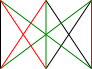
\includegraphics[height=3cm]{k33}            
    \end{center}

    Předpokládejme tedy, že $G$ je rovinný. Sestrojíme $D_G$ duální graf k $G$. Jelikož je $G$ 2-souvislý, neobsahuje mosty, tudíž $D_G$ neobsahuje smyčky. Zároveň nemůže obsahovat násobné hrany, protože to by znamenalo, že je v $G$ buď most, nebo vrchol s menším počtem vrcholů než 3 (viz následující obrázek).

    \begin{center}
        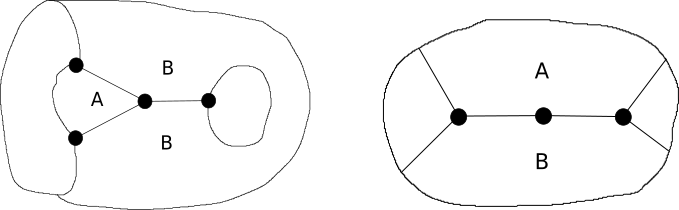
\includegraphics[height=3cm]{nasobne_hrany}
    \end{center}

    $D_G$ tedy neobsahuje smyčky ani násobné hrany. Jelikož je $G$ rovinný, je $D_G$ taktéž rovinný. Jsme tedy schopni obarvit ho pomocí nejvýše čtyř barev. Nalezneme nějaké toto obarvení s barvami $(1,2,3,4)$. Poté obarvíme hrany $D_G$ (tedy i korespondující hrany $G$) následujícím způsobem:

    \begin{itemize}
        \item Hrany mezi vrcholy 1 a 2 a mezi vrcholy 3 a 4 obarvíme barvou $a$
        \item Hrany mezi vrcholy 1 a 3 a mezi vrcholy 2 a 4 obarvíme barvou $b$
        \item Hrany mezi vrcholy 1 a 4 a mezi vrcholy 2 a 3 obarvíme barvou $c$
    \end{itemize}

    Zbývá ukázat, že toto je korektní hranové obarvení $G$. Výše jsme odargumentovali, že žádná dvojice sousedních hran nemůže sdílet obě stěny. Jelikož je ovšem stupeň vrcholů 3, musí sousední hrany sdílet alespoň jednu stěnu. Každé dvě sousední hrany tedy sdílí právě jednu stěnu. Stěny, které mají různé, navíc nemohou mít stejnou barvu, protože tyto stěny spolu sousedí přes třetí hranu vrcholu. \\

    Hrany tedy sdílí právě jednu barvu stěny. Z definice našeho obarvení ovšem plyne, že hrany stejné barvy musejí mít shodně barevné buď obě stěny, nebo žádnou. Žádné dvě sousední hrany tedy nemají stejnou barvu a naše obarvení je korektní.
    
    \section{}
    \paragraph{$2 \implies 1$}
    Relace ``být minorem'' je transitivní. Čili když $H$ je minor $G$ a $J$ je minor $H$, je $J$ zároveň minorem $G$. Z toho plyne, že pokud $H \preccurlyeq_M G$, nemůže existovat graf, který je minorem $H$, ale není minorem $G$. Jinými slovy pokud graf není minorem, nemůže být ani minorem minoru. Tím pádem pokud existuje $\mathcal{F}$ t.ž. $M = \text{Forb}(\mathcal{F})$, musí $M$ obsahovat minory všech grafů v $M$. 

    \paragraph{$1 \implies 2$}
    Mějme množinu $M$ uzavřenou vůči minorům. Vezměme $\mathcal{F}$ množinu všech grafů, které nejsou v $M$. Žádný graf z $M$ díky uzavřenosti neobsahuje žádný graf z $\mathcal{F}$ jako minor, tedy $M \subseteq \text{Forb}(\mathcal{F})$. Abychom dokázali rovnost, uvažme graf $G$ takový, že $G \in \text{Forb}(\mathcal{F})$ a zároveň $G \notin M$. \\

    Jelikož $G \notin M, G \in \mathcal{F}$. Každý graf je ovšem vlastním minorem. To nám dává spor s tím, že $G \in \text{Forb}(\mathcal{F})$. $M$ se tedy rovná $\text{Forb}(\mathcal{F})$.

    \section{}
    Dokážeme indukcí podle počtu vrcholů grafu. Graf s jedním vrcholem je $d$-degenerovaný pro všechna přirozená $d$ a má stupeň 0, tedy předpoklad splňuje. \\

    Mějme graf $G$ o $n$ vrcholech. Protože je $d$-degenerovaný, najdeme v něm vrchol $v$ stupně nejvýše $d$. Po odtržení tohoto vrcholu dostaneme graf $G'$, který je z degenerovanosti $G$ taktéž $d$-degenerovaný a obsahuje méně vrcholů. Podle indukčního předpokladu má tedy průměrný stupeň nejvýše $2d$, čili součet všech stupňů je nejvýše $2d(n-1)$. \\
    
    Přidáním $v$ zpět do grafu dostaneme navíc jeden vrchol stupně nejvýše $d$ a nejvýše $d$ vrcholům z $G'$ (sousedům $v$) zvýšíme stupeň o jedna. Průměrný stupeň grafu $G$ je tedy shora odhadnutelný jako

    \begin{align*}
        \frac{\sum \text{deg} v}{n} = \frac{2d(n-1) + d + d \cdot 1}{n} = \frac{2dn}{n} = 2d
    \end{align*}

    \section{}
    Mějme plochu $\Gamma$ s charakteristikou $\chi (\Gamma)$
    Nechť $G$ je 7-regulární graf nakreslitelný na $\Gamma$ s $n$ vrcholy, $m$ hranami a $s$ stěnami. Uvažujme $G$ souvislý. Ze 7-regularity víme $m = \frac{7}{2}n$. Zároveň víme, že obecně platí $s \leq \frac{2}{3}m$. Dosazením do Eulerova vzorce tedy dostáváme
    
    \begin{align*}
        \chi (\Gamma) &= n - m + s \\
        \chi (\Gamma) &\leq n - m + \frac{2}{3}m \\
        \chi (\Gamma) &\leq n - \frac{m}{3} \\
        \chi (\Gamma) &\leq n - \frac{7}{6}n \\
        \chi (\Gamma) &\leq -\frac{1}{6}n \\
                    n &\leq -6 \chi (\Gamma)
    \end{align*}

    Máme tedy pouze konečně mnono možností na počet vrcholů grafu. Pro libovolně zvolené $n$ pak máme nejvýše $2^{\binom{n}{2}}$ - tedy opět konečně mnoho - různých grafů. (Pro každou dvojici vrcholů vybereme, jestli mezi nimi vede hrana.) Celkový počet nakreslitelných grafů pak získáme sečtením počtů nakreslitelných grafů velikosti $n$ pro všechna možná $n$. Součtem konečného počtu konečných čísel dostaneme opět konečné číslo, tudíž celkový počet takovýchto grafů nakreslitelných na $\Gamma$ je konečný.\\

    Pokud by $G$ nebyl souvislý, skládá se z konečného počtu souvislých komponent, přičemž v každé komponentě máme z předchozího na výběr jen z konečného množství souvislých grafů. Dosazováním z konečně mnoha možností na konečné množství pozic dostaneme opět jen konečně mnoho možností, tudíž tvrzení platí i pro nesouvislé grafy.

    \section{}
    Dokážeme indukcí podle počtu vrcholů. Pro jednobarevné grafy platí tvrzení triviálně, neb $\binom{1}{2} = 0$. Pro $K_2$ platí taktéž, jelikož jeho vrcholová barevnost je 2 a obsahuje jednu hranu. \\

    Mějme z indukčního předpokladu graf s $k$ barvami a alespoň $\binom{k}{2}$ hranami. K tomuto grafu připojíme vrchol $v$. Pokud deg $v < k$, najdeme barvu, se kterou vrchol nesousedí, a obarvímem ho tou barvou. Jelikož jsme pouze přidali hrany a nezvýšili barevnost, tvrzení platí. \\

    Předpokládejme tedy, že deg $v = k$ a navíc má každý soused $v$ jinou barvu. V tom případě obarvíme $v$ barvou $k+1$. Dostaneme tedy graf s barevností $k+1$ a počtem hran alespoň

    \begin{align*}
        \binom{k}{2} + k = \frac{k(k-1)}{2} + k = \frac{k(k-1) + 2k}{2} = \frac{k(k+1)}{2} = \binom{k+1}{2},
    \end{align*}

    tedy tvrzení stále platí. Pro deg $v > k$ je argument stejný, neb jsme jen přidali další hrany navíc, čímž nerovnost neporušíme.
    \end{document}